\documentclass[a4paper,american]{paper}
\usepackage[T1]{fontenc}
\usepackage[utf8]{inputenc}
\pagestyle{plain}
\usepackage{babel}
\usepackage{textcomp}
\usepackage[mathscr]{euscript}
\usepackage{amsmath}
\usepackage{amsthm}
\usepackage{setspace}
\usepackage[unicode=true]{hyperref}
\usepackage{breakurl}
\usepackage{txfonts}
\usepackage{pxfonts}
\usepackage{tikz}
\usetikzlibrary{arrows.meta,positioning,calc}
\usepackage{tkz-graph}
\usepackage{graphicx}
\usepackage{float}
\usepackage{needspace}
\usepackage[left=3.5cm,right=3.5cm]{geometry}

\graphicspath{ {./images/} }
\date{\today}

\makeatletter
\providecommand*{\code}[1]{\texttt{#1}}
\makeatother

\counterwithin*{equation}{section}
\counterwithin*{equation}{subsection}

\theoremstyle{definition}\newtheorem{definition}{Definition}
\hyphenation{counterfactual}
\hyphenation{possible}
\hyphenation{worlds}
\hyphenation{model}
\hyphenation{structure}

\begin{document}

\title{An interactive demonstration of counterfactual truth conditions}

\subtitle{Bachelor Thesis}

\author{%
	Andreas Paul Bruno Lönne\\
	\code{\href{mailto:loenne@campus.tu-berlin.de}{loenne@campus.tu-berlin.de}}
}

\institution{
	Technische Universität Berlin\\discourse
	Degree program: Bachelor Informatik / Computer Science
}

\maketitle

\begin{abstract}
In this thesis, I address the scarcity of online resources, showcasing counterfactual truth conditions in an intuitive and digestible manner. To this end I (i) formulate a semantic satisfiability game for counterfactual sentences; (ii) prove its correctness; (iii) prove that it always halts after a finite number of moves; (iv) develop a browserbased web-application, that makes the semantic game of counterfactuals playable.
\end{abstract}
\section{Lewis' counterfactual operators}
With these introductory thoughts out of the way, let us talk in greater detail about the counterfactual operators themselves. Lewis introduces the counterfactual would $\boxright$ and counterfactual might $\Diamondright$ operators as binary modal operators. \cite{lewis_counterfactuals_1973} When we write $\varphi\boxright\psi$, we call the formula $\varphi$ the antecedent and the formula $\psi$ the consequent. We may informally rewrite one of our former examples as "I~did~not~forget~about~my~appointment~$\boxright$~I~was~punctual" and read it the following way. Read $\varphi\boxright\psi$ as "If it were the~case that $\varphi$, then it would be the case that $\psi$", and read $\varphi\Diamondright\psi$ as "If it were the case that~$\varphi$, then~it might be the case that $\psi$".\\
\subsection{Lewis' system of spheres}
The truth conditions of the counterfactual operators are stated with respect to a structure, called a \textit{system~of~spheres}. Lewis defines a system~of~spheres as follows.
\begin{figure}[H]
	Let $\$$ be an assignment to each possible world $i$ of a set $\$_i$ of sets of possible worlds. Then $\$$ is called a (centered) system of spheres, and the members of each $\$_i$ are called spheres around $i$, if and only if, for each world $i$, the following conditions hold.
	\begin{itemize}
	\item[(C)] $\$_i$ is centered on $i$; that is, the set $\{i\}$ having $i$ as its only member belongs to $\$_i$.
	\item[(1)] $\$_i$ is nested; that is, whenever $S$ and $T$ belong to $\$_i$, either $S$ is included in $T$ or $T$ is included in $S$.
	\item[(2)] $\$_i$ is closed under unions; that is, whenever $\mathscr{S}$ is a subset of $\$_i$ and $\bigcup\mathscr{S}$ is the set of all worlds $j$ such that $j$ belongs to some member of $\mathscr{S}$, $\bigcup\mathscr{S}$ belongs to $\$_i$.
	\item[(3)] $\$_i$ is closed under (nonempty) intersections; that is, whenever $\mathscr{S}$ is a nonempty subset of $\$_i$ and $\bigcap\mathscr{S}$ is the set of all worlds $j$ such that $j$ belongs to every member of $\mathscr{S}$, $\bigcap\mathscr{S}$ belongs to $\$_i$.
	\end{itemize}
	\caption{Lewis' system of spheres}
	\label{fig:system_of_spheres}
\end{figure}
\noindent Now let us first take a broad perspective upon this definition. Most generally a system of spheres is an assignment of a set of sets of possible worlds to each world. The assigned sets exhibit the four characteristics (C), (1), (2) and (3); and are called sets of spheres. In totality such a system of spheres serves to codify the relationships of accessibility and comparative~similarity between possible worlds. To this end each set of spheres describes an ordering of possible worlds with respect to similarity to the world it is assigned to. Meaning, that the set of spheres $\$_i$ describes the comparative~similarity to- and accessibility from $i$ for each world. This is briefly illustrated by the next example.

\begin{figure}[H]
\centering
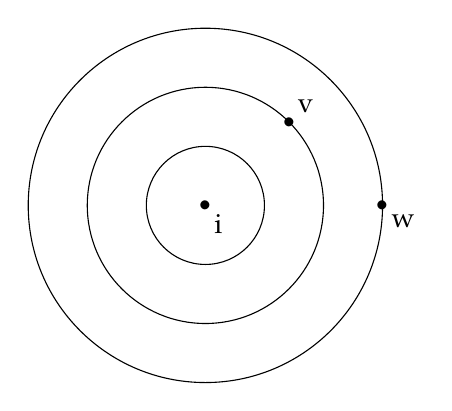
\begin{tikzpicture}[
roundnode/.style={circle, draw=black!0, fill=black!100, very thick, minimum size=1pt},
]
\coordinate (O) at (0,0);
\coordinate (V) at (45:1.5);
\coordinate (W) at (0:2.25);
\draw (O) circle (2.25);
\draw (O) circle (1.5);
\draw (O) circle (0.75);
\node[scale=1mm, label={[label distance=-6mm]315:i}] at (O) {.};
\node[scale=1mm, label={[label distance=-6mm]45:v}] at (V) {.};
\node[scale=1mm, label={[label distance=-6mm]315:w}] at (W) {.};

%\draw[black] (0,0) -- (1,0);
\end{tikzpicture}
\caption{A set of spheres $\$_i=\{\{ i\} ,\{ i,v\} ,\{ i,v,w\}\}$}
\label{fig:set_of_spheres}
\end{figure}

\noindent In this example we look at the worlds $i$, $v$ and $w$; and consider the set of spheres $\$_i$. The spheres themselves are sets of possible worlds and are visualized through circles. A world inside or on the circumference of a circle is contained within the corresponding sphere. Crucially, the meaning of a sphere around $i$ is that each world contained in it is more similar to $i$ than each world not contained in it. For our example this means that $i$ is more similar to itself than any other world; $i$ and $v$ are more similar to $i$ than any other world; and that $i$, $v$ and $w$ are more similar to $i$ than any other world. Regarding accessibility, a world is said to be accessible from $i$, if it is contained in any sphere around $i$. So we can see that all $i$, $v$ and $w$ are accessible from $i$. With this in mind, we can motivate the properties (C), (1), (2) and (3).\\

(C) It seems reasonable to assume that each world is most similar to itself and that there cannot be another world equally or more similar to it than itself. If that is the case, every sphere around a world $i$ needs to contain the set $\{ i\}$.\\
\indent (1) Intuitively it may also make sense, that for each pair of spheres around the same world one should include the other. If we entertain the notion, that the spheres around a world are not nested, then one of those spheres cannot be a sphere. First, remember that a sphere around a world $i$ is a set of possible worlds, such that each world contained in it is more similar to $i$, than every world not contained in it. Then suppose the set of spheres $\$_i$ is not nested. In that case two worlds $v$ and $w$ and the spheres $S,T\in\$_i$ exist, such that $v\in S$, $w\notin S$, $v\notin T$ and $w\in T$. Through $S$ we know that that $v$ is more similar to $i$ than $w$. And through $T$ we know that that $w$ is more similar to $i$ than $v$. Which cannot both be the case at the same time.\\
\indent (2) Suppose that for the union $\bigcup\mathscr{S}$ of a set of spheres $\mathscr{S}$ around $i$, there are two worlds $v,w$ such that $v\in\bigcup\mathscr{S}$ and $w\notin\bigcup\mathscr{S}$. Then that means, that $v$ is, and $w$ is not, contained in some sphere in $\mathscr{S}$. Hence $v$ is more similar to $i$ than $w$. Therefore $\bigcup\mathscr{S}$ is a set such that any world contained within it is more similar to $i$ than any world not contained in it. We call such a set a sphere around $i$.\\
\indent (3) Suppose that for the intersection $\bigcap\mathscr{S}$ of a nonempty set of spheres $\mathscr{S}$ around $i$, there are two worlds $v,w$ such that $v\in\bigcap\mathscr{S}$ and $w\notin\bigcap\mathscr{S}$. Then that means, that $v$ is, and $w$ is not, contained in some sphere in $\mathscr{S}$. Hence $v$ is more similar to $i$ than $w$. Therefore $\bigcap\mathscr{S}$ is a set such that any world contained within it is more similar to $i$ than any world not contained in it. We call such a set a sphere around $i$.
\subsection{Lewis' counterfactual truth conditions}
Then let us take a look at Lewis' counterfactual truth conditions. Take the counterfactual operators as part of some logic, where formulas like $\varphi$ and $\psi$ are evaluated with respect to some world and a system of spheres. Lewis abbreviates a world, where the formula $\varphi$ holds as a $\varphi$-world. The truth conditions of Lewis' counterfactual would operator are these.
\begin{figure}[H]
	\centering
	$\varphi\boxright\psi$ is true at a world i (according to a system of spheres \$) if and only if either
	\begin{itemize}
	\item[(1)] no $\varphi$-world belongs to any sphere $S$ in $\$_i$, or
	\item[(2)] some sphere $S$ in $\$_i$ does contain at least one $\varphi$-world, and $\varphi\rightarrow\psi$ holds at every world in $S$.
	\end{itemize}
	\caption{Lewis' counterfactual would truth conditions}
	\label{fig:counterfactual_would}
\end{figure}
\noindent The counterfactual would evaluates to true iff either (1) or (2) is true.\\
\indent (1) We describe the first case as vacuous truth. Intuit this case the same way a material implication is true, when its antecedent is false. From wrong antecedents arbitrary consequents may be inferred. Keep in mind however, that the vacuous truth of the counterfactual would is much stricter. While the material conditional only requires the antecedent to be false at the world it is evaluated at, the counterfactual would requires the antecedent to be false at every accessible world.\\
\indent (2) The non-vacuous case requires the existence of a sphere throughout which $\varphi\rightarrow\psi$ holds and that that sphere also contains a $\varphi$-world. The existence of such a sphere can roughly be understood as the existence of some accessibility restriction under which the strict conditional $\Box (\varphi\rightarrow\psi)$ comes out as non-vacuously true. Meaning that $\varphi\rightarrow\psi$ holds throughout all accessible worlds and that at least one accessible world is a $\varphi$-world. While the strict conditional is true, only if it is true in the broadest sense---meaning it is true at every accessible world---the counterfactual would conditional merely needs to be true in one of many senses. That is why Lewis' counterfactual operators are called variably strict conditionals. Each of these many senses are degrees of similarity to a world, that are described by spheres around that world. To motivate why overall similarity between worlds is used as an accessibility restriction consider this example.
\begin{equation}
\text{"If Kennedy had pressed the red button, there would have been nuclear war"}
\end{equation}
We consider this to be true. Without much trouble, one can make up many counterexamples to this counterfactual. Imagine for a moment the possibility that Kennedy had pressed the red button and the button malfunctioned. In that case Kennedy pressed the button, but there is no nuclear war. Obviously that is not meant. When we say something like "If~it~were~the~case that A, then it would be the case that B", we implicitly mean "If it were the case that~A and things were pretty much as they are otherwise, then it would be the case that~B". Our rebuttal therefore may be that there is at least one possible world where Kennedy pressed the red button and the red button did not malfunction that is more similar to the actual world than any possible world where Kennedy pressed the red button and the button did malfunction. If this is the case, we may claim that our example counterfactual is true, although there are certain senses in which it is not true. This is why a counterfactual would operator is true, if there is at least one sense, represented through a sphere of accessibility, in which it is true. Regarding the system of spheres it means that a counterfactual would operator is non-vacuously true, unless each sphere around the world it is evaluated at contains a refuting world that serves as a counterexample or no sphere around the world it is evaluated at contains a $\varphi$-world.\\
The \textit{counterfactual~might} is defined analogously.

\begin{figure}[H]
	\centering
	$\varphi\Diamondright\psi$ is true at a world i (according to a system of spheres \$) if and only if both
	\begin{itemize}
	\item[(1)] some $\varphi$-world belongs to some sphere $S$ in $\$_i$, and
	\item[(2)] every sphere $S$ in $\$_i$ that contains at least one $\varphi$-world contains at least one world where $\varphi\wedge\psi$ holds.
	\end{itemize}
	\caption{Lewis' counterfactual might truth conditions}
	\label{fig:counterfactual_might}
\end{figure}

\noindent Note the differences in quantification and truth conditions. The counterfactual would's existential quantifier for the existance of a sphere is replaced by a universal quantifier requiring every sphere containing a $\varphi$-world to also contain a $(\varphi\wedge\psi)$-world. While the counterfactual would requires each world of a sphere to fulfill its criteria, the counterfactual might requires one world of each sphere, that contains a $\varphi$-world, to fulfill its criteria. Notice also that the counterfactual might does not have two separate truth cases and is true in only one case. But since the counterfactual would and counterfactual might are interdefinable, we wont go into further detail here.
\begin{equation}
\varphi\boxright\psi = \neg (\varphi\Diamondright\neg\psi )
\end{equation}
\begin{equation}
\varphi\Diamondright\psi = \neg (\varphi\boxright\neg\psi )
\end{equation}

\section{Counterfactual logic}
This section is concerned with defining counterfactual logic. First it provides a brief definition of well-formed counterfactual formulas, then introduces the structure they are evaluated on and concludes by defining the truth conditions of counterfactual logic.

\subsection{Counterfactual formulas}
We call $\Phi = \{\varphi ,\psi ,...\}$ the set of all well-formed counterfactual formulas.
\begin{definition}[Well-formed counterfactual formula]
Given an infinite set of atomic formula symbols $Atoms = \{ x, y, ...\}$ and an alphabet $A~=~\{\bot ,\top ,\neg ,\vee ,\wedge ,\Diamond ,\Box ,\boxright ,\Diamondright\}\cup Atoms$, the structure of every well-formed counterfactual formula is expressed through the following Backus-Naur form.
\begin{equation}
\varphi, \psi ::= \bot \mid \top \mid x \mid \neg \varphi \mid \varphi \vee \psi \mid \varphi \wedge \psi \mid \Diamond \varphi \mid \Box \varphi \mid \varphi \boxright \psi \mid \varphi \Diamondright \psi
\end{equation}
\end{definition}

\subsection{Counterfactual~kripke~structure}
In order to evaluate the non-truth-functional connectives of counterfactual~logic, we define a variation of the Kripke~structure in \cite{kripke_modal_logic_1963}. To evaluate Lewis' counterfactual truth conditions \cite{lewis_counterfactuals_1973}, we also introduce a notion of similarity between possible worlds to the accessibility relation.
\begin{definition}[counterfactual kripke structure]
A {\it counterfactual kripke structure} is an ordered triple $(W, \leadsto ,F)$, where $W=\{w,v,...\}$ is the set of all possible~worlds, $\leadsto \colon W\times \mathbb{R} \times W$ is the similarity relation, and $F \colon W \rightarrow 2^{Atoms}$ is an assignment of each world, to a set of atomic formulas.
\end{definition}
\noindent Let us explain further the members of our counterfactual~kripke~structure.\\
The set of all possible~worlds $W$ represents all complete and self-consistent ways reality could have been. $F$ in turn, describes the state of affairs at each world. It assigns to each world a set of atomic propositions, that are the case at it. The similarity relations purpose is twofold. It serves as an accessibility relation, restricting accessibility between worlds and also carries information about comparative similarity between worlds. In particular this means for any two worlds $w$ and $v$, that iff $w\overset{r}{\leadsto} v$, then $v$ is called accessible from $w$. $w\overset{r}{\leadsto} v$ also means, that $r$ is a measure of similarity between $w$ and $v$, from the standpoint of $w$. We can suppose another world $v'$, with $w\overset{r'}{\leadsto} v'$ and compare $r$ and $r'$. If $r < r'$, we can conclude, that $v$ is more similar to $w$ than $v'$, from the standpoint of $w$. Additionally we note, that for our purposes $\leadsto$ will always contain a tuple $(w, 0, w)$ for each world $w\in W$. This is because we assume analogously to Kripke, that worlds are self-similar and are accessible from themselves. Finally we introduce $W_w = \{w'\mid w \overset{r}{\leadsto} w'\}$ as a shorthand for the set of all accessible worlds, from a world $w$.
%\newpage
\subsection{Truth conditions of counterfactual logic}
Given a counterfactual~kripke~structure $S = (W, \leadsto ,F)$ and a world $w$,\\
$S,w\nvDash\bot$.\\
$S,w\vDash\top$.\\
$S,w\vDash x$ iff $x\in F(w)$.\\
$S,w\vDash \neg\varphi$ iff $S,w\nvDash\varphi$.\\
$S,w\vDash \varphi\vee\psi$ iff ($S,w\vDash\varphi$ or $S,w\vDash\psi$).\\
$S,w\vDash \varphi\wedge\psi$ iff ($S,w\vDash\varphi$ and $S,w\vDash\psi$).\\
$S,w\vDash \Diamond \varphi$ iff a world $w'\in W_w$ exists, such that $S,w' \vDash \varphi$.\\
$S,w\vDash \Box \varphi$ iff for every world $w'\in W_w$, it is true that $S,w' \vDash \varphi$.\\
$S,w \vDash \varphi \boxright \psi$, iff either
\begin{itemize}
	\item[(1)] no world $w'\in W_w$ exists, such that $S,w' \vDash \varphi$, or
	\item[(2)] a world $w'$ and an $r$ exist, such that $w\overset{r}{\leadsto} w'$ and $S,w'\vDash \varphi$ and for each world $w^*$, for which an $r^*$ exists, such that $r^*\leq r$ and $w\overset{r^*}{\leadsto} w^*$, it is true that $S,w^*\vDash\neg\varphi\vee\psi$.
\end{itemize}
\noindent$S,w\vDash \varphi \Diamondright \psi$, iff both 
\begin{itemize}
	\item[(1)] a world $w'\in W_w$ exists, such that $S,w' \vDash \varphi$, and
	\item[(2)] for every world $w''$, for which an $r''$ exists, such that $w\overset{r''}{\leadsto}w''$ and $S,w'' \vDash \varphi\wedge\neg\psi$ are true, a world $w^*$ and an $r^*$ exist, such that $r^* \leq r''$ and $w\overset{r^*}{\leadsto}w^*$ and $S,w^* \vDash \varphi\wedge\psi$.
\end{itemize}
\section{The semantic game of counterfactuals}
This section offers an overview and introduction to the semantic~game~of~counterfactuals. The semantic~game~of~counterfactuals is a sequential two-player reachability game, wherein a \textit{defender} $d$ tries to prove a counterfactual formula and an \textit{attacker} $a$ tries to disprove it. The defender begins the game as the \textit{active~player}, with a counterfactual~formula at a possible~world. The active player is a role assigned to the player that can currently make moves and whose typical objective it is to prove the current formula through play. As the active player makes moves, the counterfactual formula is resolved progressively until a player resolves a $\top$ and wins; or cannot make any move and loses. Throughout the game, moves may change the active player and current world.

\subsection{Definition of the semantic game}
The game is akin to a discussion where players make arguments and refute them. Weak arguments do not hold up to scrutiny, but strong ones do. The players' adversarial interplay allows the discovery and dismissal of arguments, such that the reason for truth or falsity of a claim is revealed. Of course, this is only possible when the players make the best possible moves. We shall call such play optimal play. We describe the game the following way.
\begin{definition}[Semantic game of counterfactuals]
The semantic game of counterfactuals $\mathfrak{S}[\varphi ,w,S]=(I, E, G, R)$ with respect to a formula $\varphi$, a world $w$ and a counterfactual kripke structure $S=(W,\leadsto ,F)$ is an ordered tuple consisting of
\begin{itemize}
\item an initial game state $I=(\varphi ,w)_d$
\item a set of winning game states $E=\{(\top ,w)_p \mid w\in W\wedge p\in\{ a,d\}\}$
\item a set of all game states $G$
\item and a transition relation $R: G\times G$
\end{itemize}
The notation $\mathfrak{S}_p[\varphi ,w,S]$ means that the annotated player $p\in\{a,d\}$ begins the game; that is, $I=(\varphi ,w)_p$ instead of $I=(\varphi ,w)_d$.
\end{definition}
The initial game state $I$ varies from game to game. It contains the formula $\varphi$ that ought to be proven and the world $w$ it ought to be proven at. It is always indexed by the initial active player, that is the defender. The set of winning game states contains all game states in which the active player wins. When the active player wins, the respective other player loses. The set $E$ includes all game states where the formula is resolved to a $\top$-symbol. It is also possible for a player to win without reaching a winning game state. This is the case when the active player is unable to make a move and is stuck. When this happens, the active player loses and the active player's opponent i.e. the inactive player wins. $\mathfrak{S}[\varphi ,w,S]$ also contains the set of all game states $G$ and the set $R$ of transitions between game states which we call moves. In later sections we will define two such sets of moves. One general formulation $\rightarrow$ and one simplified formulation $\rightarrow_l$ employing the limit assumption. One may take either as $R$. In order to arrive at our definition for $\rightarrow$ and $\rightarrow_l$, let us first define game states and transitions.

\subsection{Game states}
Game states form the backbone of the semantic game of counterfactuals by describing its game positions. Each game state describes the game at a discrete point in time in-between moves.
\begin{definition}[Game state]
A game state is a tuple that can take any one of the forms
\begin{itemize}
	\item[(1)] $(\varphi ,w)_p$
	\item[(2)] $(\varphi ,w, e)_p$
	\item[(3)] $(\varphi ,w,w',r)_p$
\end{itemize}
where $\varphi\in\Phi$; $w,w'\in W$; $r\in\mathbb{R}$ and $p,e\in\{ a,d\}$.
\end{definition}
\noindent Of these types of game states (1) is the most common. It carries a counterfactual formula, the current world and is indexed with the active player. It is employed to resolve atomic formulas $x,y,...$ and the propositional symbols $\top,\neg,\vee,\Diamond$; while also serving as an initial and final state type for other resolutions. (2) is a type of game state that represents a player temporarily becoming active and choosing a state transition. $e$ holds the previous active player, which will resume being active after the next state transition. Lastly, game~state~type~(3) is an extension of~(1), describing a game state where a sphere~of~accessibility has been chosen. $w'$ is a \textit{sphere-delimiting~world}, lying exactly on the surface of said sphere~of~accessibility with radius $r$. We will look at this in further detail in the next subsection.\\

\subsection{Moves}
When the active player transforms the current game state into another and progresses the game, we call that a move. Formally we represent this through a tuple of game states.
\begin{definition}[Move]
A move $m$ is a tuple $m\in G\times G$.
\end{definition}
\noindent The first element of the tuple is the initial game state, while the second one is the resulting game state. We define the set of moves $\rightarrow$ specific to the semantic~game~of~counterfactuals.
\begin{definition}[Moves]\label{def:set_moves}
$\rightarrow$ is a set of moves, such that it contains exactly those tuples that fit any of the forms described by the following 19 types of moves. For each of those types of moves variables are quantified separately. Additionally, square brackets above the relation symbol are used to annotate restrictions imposed upon the quantification of those variables. In case of (1) for example $x$ is restricted to range across atomic formulas contained in $F(w)$. Furthermore, it is always true that $\varphi ,\psi\in\Phi$ are counterfactual formulas; $x\in Atoms$ is an atomic formula; $w,w',w^*\in W$ are worlds; $p,e\in\{ a,d\}$ are players; $np\in\{ a,d\}\setminus{}\{ p\}$ is the opponent of the player p; and $r,r^*\in\mathbb{R}$.
\begin{figure}[H]
	\centering
	\begin{equation}
		(x ,w)_{p}\xrightarrow{[x\in F(w)]} (\top ,w)_{p}
	\end{equation}
	\begin{equation}
		(\neg\varphi ,w)_{p}\rightarrow (\varphi ,w)_{np}
	\end{equation}
	\begin{equation}
		(\varphi\vee\psi ,w)_{p}\rightarrow (\varphi ,w)_{p}
	\end{equation}
	\begin{equation}
		(\varphi\vee\psi ,w)_{p}\rightarrow (\psi ,w)_{p}
	\end{equation}
	\begin{equation}
		(\varphi\wedge\psi ,w)_{p}\rightarrow (\varphi\wedge\psi ,w,p)_{np}
	\end{equation}
	\begin{equation}
		(\varphi\wedge\psi ,w,e)_{p}\rightarrow (\varphi ,w)_{e}
	\end{equation}
	\begin{equation}
		(\varphi\wedge\psi ,w,e)_{p}\rightarrow (\psi ,w)_{e}
	\end{equation}
	\begin{equation}
		(\Diamond\varphi ,w)_{p}\xrightarrow{[w\overset{r}{\leadsto}w']} (\varphi ,w')_{p}
	\end{equation}
	\begin{equation}
		(\Box\varphi ,w)_{p}\rightarrow (\Box\varphi ,w,p)_{np}
	\end{equation}
	\begin{equation}
		(\Box\varphi ,w,e)_{p}\xrightarrow{[w\overset{r}{\leadsto}w']} (\varphi ,w')_{e}
	\end{equation}
	\begin{equation}
		(\varphi\boxright\psi ,w)_p\rightarrow (\Box\neg\varphi ,w)_{p}
	\end{equation}
	\begin{equation}
		(\varphi\boxright\psi ,w)_p\xrightarrow{[w\overset{r}{\leadsto}w']}(\varphi\boxright\psi ,w,w',r)_{np}
	\end{equation}
	\begin{equation}
		(\varphi\boxright\psi ,w,w',r)_p\rightarrow (\varphi ,w')_{np}
	\end{equation}
	\begin{equation}
		(\varphi\boxright\psi ,w,w',r)_p\xrightarrow{[w\overset{r^*}{\leadsto}w^*,r^*\leq r]}(\neg\varphi\vee\psi ,w^*)_{np}
	\end{equation}
	\begin{equation}
		(\varphi\Diamondright\psi ,w)_p\rightarrow (\varphi\Diamondright\psi ,w,p)_{np}
	\end{equation}
	\begin{equation}
		(\varphi\Diamondright\psi ,w,e)_{p}\rightarrow (\Box\neg\varphi ,w)_{p}
	\end{equation}
	\begin{equation}
		(\varphi\Diamondright\psi ,w,e)_p\xrightarrow{[w\overset{r}{\leadsto}w']}(\varphi\Diamondright\psi ,w,w',r)_{e}
	\end{equation}
	\begin{equation}
		(\varphi\Diamondright\psi ,w,w',r)_p\rightarrow (\varphi ,w')_{np}
	\end{equation}
	\begin{equation}
		(\varphi\Diamondright\psi ,w,w',r)_p\xrightarrow{[w\overset{r^*}{\leadsto}w^*,r^*\leq r]}(\varphi\wedge\psi ,w^*)_{p}
	\end{equation}
	\caption{Moves of the semantic game of counterfactuals}
	\label{fig:moves}
\end{figure}
\end{definition}
\noindent Each symbol of the counterfactual logic is resolved through one or more resolution steps. Take (9) and (10) for the resolution of the necessity operator as an example. The operator is resolved in two steps by first making the move (9) and then (10). Each such sequence of resolution steps both begins and ends with a game state of the form $(\varphi ,w)_p$. The meaning of this type of game state is that the active player $p$ attempts to show the formula $\varphi$ at the world $w$ through subsequent play. Accordingly, the game's moves are defined in such a way that the player $p$ wins the game with optimal play, iff $\varphi$ is true at $w$. The formula $\varphi$ is resolved top-down, by continually resolving the weakest-binding operator or atomic formula, until no further resolution is possible. Since the truth conditions of the operators of counterfactual logic depend on the truth of the subformulas they bind, a game to determine the truth of the relevant subformula---or in some cases a different formula---is played after each resolution of a counterfactual operator. For this reason all resolution sequences of all operators and atomic formulas end with the type of game state $(\varphi ,w)_p$ that describes the initial state of a new game pertaining to the truth of the formula $\varphi$. This allows us to consider the resolution sequences for each operator separately. Given the invariant that the player $p$ wins the game with optimal play from the game state $(\varphi ,w)_p$, iff $\varphi$ is true at $w$ for each subformula $\varphi$. Because players frequently switch the role of active player throughout resolution sequences, it will become cumbersome and confusing to describe players by calling them the active or inactive player. We will thus call the player that is active at the beginning of a resolution sequence the proving player and their opponent the disproving player.\\
\indent (1) Atomic formulas which are true at the current world are resolved to a $\top$-symbol. The proving player subsequently reaches the $\top$-symbol and wins the game. In any game state where the current formula is an atomic formula that is not true at the current world the proving player loses since no move is possible and they are stuck.\\
\indent (2) The negation is resolved by switching the active player. The reason for this is that the truth of the formula $\neg\varphi$ can be disproven by proving the formula $\varphi$. Thus this move switches the active~player and makes the disproving player prove the subformula $\varphi$. If they are able to do so, they win and the proving player loses. Otherwise they lose and the proving player wins the game.\\
\indent (3), (4) The disjunction is resolved through the proving player's choice of which subformula to prove i.e. the choice to make the move (3) or (4). If one of the subformulas is true, then the proving player can choose it, prove it through further play and win. In any other case the proving player loses with further optimal play.\\
\indent (5), (6), (7) Conjunctions are resolved by making the disproving player temporarily become the active player and resolve the conjunction as if it were a disjunction. In other words, the disproving player becomes active and chooses which subformula the proving player has to prove through play, before becoming inactive again. With optimal play the disproving player chooses the harder subformula for their opponent to prove. If one of the subformulas cannot be proven through play, the disproving player chooses it and wins subsequently with optimal play. Conversely if such a subformula does not exist.\\
\indent (8) The possibility operator is resolved by having any accessible world become the new current world. The proving player gets to choose that world and has to subsequently prove through play that the subformula $\varphi$ is true at it. If there exists any accessible $\varphi$-world, then the proving player can choose that world, show $\varphi$ there through play and win the game. If no such world exists, the proving player has to choose a world $\varphi$ cannot be proven at and loses subsequently with optimal play.\\
\indent (9), (10) The resolution of the necessity operator relates to the resolution of the possibility operator in a similar way as the resolution of conjunctions relates to the resolution of disjunctions. Both employ a paradigm where the relationship of duality with another operator is used by switching the active player and resolving it like their respective counterpart operator. First the disproving player becomes temporarily active (9), resolves necessity as if it were possibility (10), becomes inactive again and leaves the proving player to prove the subformula $\varphi$ at the chosen world. This is because necessity is true, when it's supposition is true at all accessible worlds. Thus the disproving player makes the worst choice in the proving player's stead. If there exists any accessible world at which the subformula $\varphi$ is not true, it is sure to be chosen with optimal play. The proving player then cannot prove $\varphi$ there through play and loses the game. If $\varphi$ is true at every accessible world however, then no world can be chosen, such that the proving player cannot prove $\varphi$ there through play. The proving player wins the game with optimal play in that case.\\
\indent (11), (12), (13), (14) Sticking closely to the structure of Lewis' definition the counterfactual would's truth conditions, the proving player first decides which truth condition---vacuous or non-vacuous truth---to claim truth of and force their opponent to attempt to disprove. Move type (11) is the choice of vacuous truth and (12) non-vacuous truth. When the proving player claims vacuous truth, they are required to prove the formula $\Box\neg\varphi$. This means that every accessible world has to not be a $\varphi$-world. If an accessible $\varphi$-world exists, the disproving player can choose it as per $\Box$, become the active player as per $\neg$, then prove $\varphi$ there and win the game. If no such world exists, the disproving player will fail to prove $\varphi$ with optimal play and lose.\\
\indent When deciding to claim that the counterfactual would in question is non-vacuously true, the initial active player also chooses a sphere of accessibility around the current world that is meant to prove non-vacuous truth. This sphere has to contain at least one $\varphi$-world and throughout each world within it $\varphi\rightarrow\psi$ has to hold. For the semantic game we adopt a slightly different but unequivocally equivalent condition. We give a sphere around a world $i$ through a world that is a most dissimilar world to $i$ still contained within the sphere. We call such a world a sphere-delimiting or delimiting world. We say that the chosen sphere's delimiting world has to be a $\varphi$-world and that $\varphi\rightarrow\psi$ has to hold throughout each world of that sphere. We know that whenever there is a sphere containing a $\varphi$-world throughout which $\varphi\rightarrow\psi$ holds, then there also is a subset of that sphere that is a sphere with a delimiting $\varphi$-world throughout which $\varphi\rightarrow\psi$ holds. We can simply take the $\varphi$-world of the former sphere as the delimiting world for the latter. And whenever there is a sphere with a delimiting $\varphi$-world throughout which $\varphi\rightarrow\psi$ holds, then that sphere is also a sphere containing a $\varphi$-world throughout which $\varphi\rightarrow\psi$ holds. Now that we have introduced the semantic game's notion of the counterfactual would's non-vacuous truth, let us explain the corresponding moves (13) and (14). After the proving player's choice to claim that the counterfactual is non-vacuously true, the disproving player chooses in which way to attempt to disprove that claim. They can claim that the chosen sphere-delimiting world is not a $\varphi$-world (13) and force the initial active player to subsequently prove it through play. Or they can assert that $\varphi\rightarrow\psi$ does not hold throughout the chosen sphere (14) and choose a world serving as a counterexample. The proving player then has to prove that $\varphi\rightarrow\psi$ holds at that world by proving through play that $\neg\varphi\vee\psi$ holds at it.\\
\indent (15), (16), (17), (18), (19) In a similar vain to the conjunction and necessity, the counterfactual might's resolution hinges on it's interdefinability with the counterfactual would. Since the interdefinition of the counterfactual would and might contains two negations however, it's resolution sequence does not show such a clear correspondence of the counterfactual would's. The counterfactual might is resolved by switching the active player temporarily (15) until the choice between (16) and (17) has been made and follows the same structure as the resolution sequence of the counterfactual would otherwise.
\subsection{Limit Assumption}
Additionally, Lewis states the limit assumption which allows a simplification of the semantic game of counterfactuals. We will call a sphere that contains a $\varphi$-world a $\varphi$-permitting sphere.
\begin{definition}[Limit assumption]
For every world $i$ and formula $\varphi$ for which a $\varphi$-permitting sphere around $i$ exists, there is a smallest $\varphi$-permitting sphere around $i$.
\end{definition}
In other words, a nonempty set of $\varphi$-permitting spheres around $i$ has a smallest member. Without a doubt this is true when there are only finitely many spheres around $i$. We can reassure us of that fact the following way. Given any sphere of a nonempty set of $\varphi$-permitting spheres $\$_i$ around a world $i$, we can check for each sphere in $\$_i$ whether it is smaller than that sphere. If that is the case for any sphere, we can take this sphere as our next sphere and repeat the same process for it. If we do not find a smaller sphere, then we found a smallest sphere. And since we assumed $\$_i$ to be finite, we will invariably run out of smaller spheres to find.
If we take $\$_i$ to be an infinite set however, we may find an infinite descending sequence of smaller and smaller spheres without end. In that case, we cannot find a smallest sphere, since every sphere has a sphere that is smaller than it.\\
\indent Since the spheres around $i$ are nested, one of any two spheres contains the other. It follows that the smallest sphere of a set of spheres $\$_i$, if it exists, is the intersection of all spheres of $\$_i$. This means that it is contained in all other spheres in $\$_i$. This circumstance proves quite useful to reduce the semantic game's complexity. This is because showing that a formula $\varphi$ does not hold throughout a smallest sphere around a world $i$ also shows that it does not hold throughout any larger sphere and by extension any sphere in $\$_i$. We will apply this notion to simplify the semantic game's resolution of counterfactual operators and thereby provide an alternative formulation of it by employing the limit assumption.

\subsection{Alternative moves}
\begin{definition}[Simplified moves]
$\rightarrow_l$ is a set of moves, such that it contains exactly those tuples that fit any of the forms described by the following 17 types of moves. Variables are quantified the same way as in definition \ref{def:set_moves}.
\begin{figure}[H]
	\centering
	\begin{equation}
		\label{eq:limit_ass_atom_move}
		(x ,w)_{p}\xrightarrow{[x\in F(w)]} (\top ,w)_{p}
	\end{equation}
	\begin{equation}
		(\neg\varphi ,w)_{p}\rightarrow (\varphi ,w)_{np}
	\end{equation}
	\begin{equation}
		(\varphi\vee\psi ,w)_{p}\rightarrow (\varphi ,w)_{p}
	\end{equation}
	\begin{equation}
		(\varphi\vee\psi ,w)_{p}\rightarrow (\psi ,w)_{p}
	\end{equation}
	\begin{equation}
		(\varphi\wedge\psi ,w)_{p}\rightarrow (\varphi\wedge\psi ,w,p)_{np}
	\end{equation}
	\begin{equation}
		(\varphi\wedge\psi ,w,e)_{p}\rightarrow (\varphi ,w)_{e}
	\end{equation}
	\begin{equation}
		(\varphi\wedge\psi ,w,e)_{p}\rightarrow (\psi ,w)_{e}
	\end{equation}
	\begin{equation}
		(\Diamond\varphi ,w)_{p}\xrightarrow{[w\overset{r}{\leadsto}w']} (\varphi ,w')_{p}
	\end{equation}
	\begin{equation}
		(\Box\varphi ,w)_{p}\rightarrow (\Box\varphi ,w,p)_{np}
	\end{equation}
	\begin{equation}
		(\Box\varphi ,w,e)_{p}\xrightarrow{[w\overset{r}{\leadsto}w']} (\varphi ,w')_{e}
	\end{equation}
	\begin{equation}
		(\varphi\Diamondright\psi ,w)_{p}\xrightarrow{[w\overset{r}{\leadsto}w']} (\varphi\Diamondright\psi ,w,w',r)_{np}
	\end{equation}
	\begin{equation}
		(\varphi\Diamondright\psi ,w,w',r)_{p}\rightarrow (\varphi\wedge\psi ,w')_{np}
	\end{equation}
	\begin{equation}
		(\varphi\Diamondright\psi ,w,w',r)_{p}\xrightarrow{[w\overset{r^*}{\leadsto}w^*, r^*<r]} (\neg\varphi ,w^*)_{np}
	\end{equation}
	\begin{equation}
		(\varphi\boxright\psi ,w)_{p}\rightarrow (\varphi\boxright\psi ,w,p)_{np}
	\end{equation}
	\begin{equation}
		(\varphi\boxright\psi ,w,e)_{p}\xrightarrow{[w\overset{r}{\leadsto}w']} (\varphi\boxright\psi ,w,w',r)_{e}
	\end{equation}
	\begin{equation}
		(\varphi\boxright\psi ,w,w',r)_{p}\rightarrow (\neg\varphi\vee\psi ,w')_{p}
	\end{equation}
	\begin{equation}
		(\varphi\boxright\psi ,w,w',r)_{p}\xrightarrow{[w\overset{r^*}{\leadsto}w^*, r^*<r]} (\varphi ,w^*)_{p}
	\end{equation}
	\caption{Moves employing the limit assumption}
	\label{fig:limit_ass_moves}
\end{figure}
\end{definition}
Moves (1)-(10) are the same as in the formulation in figure \ref{fig:moves}.\\
\indent (11), (12), (13) With respect to the limit assumption, we can formulate a simpler resolution of the counterfactual might. It can be proven by showing that the smallest $\varphi$-permitting sphere around the current world $w$ does contain a $(\varphi\wedge\psi )$-world. In that case every larger sphere around $w$ also contains a $(\varphi\wedge\psi )$-world; and every smaller sphere around $w$ does not contain a $\varphi$-world. This corresponds to the requirement (2) of Lewis' truth conditions of the counterfactual might (see figure \ref{fig:counterfactual_might}). Furthermore, it is necessary to show that a $\varphi$-permitting sphere around $w$ exists. Hence the counterfactual might's resolution sequence begins with the proving player's choice of a sphere of accessibility (11). When the proving player cannot choose a sphere, because no other world is accessible, they lose. In that case, no $\varphi$-permitting sphere around $w$ exists. In the case that the proving player is able to choose a sphere-delimiting world and thus a sphere, the chosen world ought to be a $(\varphi\wedge\psi )$-world. This is because we combine two truth requirements that the sphere needs to contain a $\varphi$-world; and that the sphere needs to contain a $(\varphi\wedge\psi )$-world. If the latter is true, the former is true as well. Thus we can omit the less stringent requirement. Analogously to the previous formulation of the counterfactual would's resolution, we assert without loss of generality that the chosen sphere be $(\varphi\wedge\psi )$-delimited instead of merely containing a $(\varphi\wedge\psi )$-world. If the proving player did not choose a $(\varphi\wedge\psi )$-world, then the disproving player is able to refute that by forcing the proving player to prove $(\varphi\wedge\psi )$ at the chosen world (12). If the delimiting world is either not a $\varphi$-world or not $(\varphi\wedge\psi )$-world, then the proving player loses subsequently with optimal play. And if there exists a smaller $\varphi$-permitting sphere than the sphere chosen by the proving player, then that players opponent can choose a closer world and force the proving player to attempt to show through play that the chosen world is not a $\varphi$-world (13). If it is a $\varphi$-world, then the proving player loses with optimal play and wins otherwise.\\
\indent (14), (15), (16), (17) The counterfactual would is resolved by switching the active player before and after the choice of a sphere of accessibility and resolving it similarly to a counterfactual might. First, the active player is switched (14). Then the disproving player chooses a sphere of accessibility (15). And finally the proving player becomes active again and chooses in which way to disprove the disproving players chosen sphere. The proving player may either prove that $\varphi\rightarrow\psi$ holds at the chosen sphere-delimiting world by proving that $\neg\varphi\vee\psi$ holds there (16) or they may prove that there is a smaller $\varphi$-permitting sphere by proving that there is a more similar $\varphi$-world (17).

\bibliographystyle{alphaurl}
\bibliography{thesis}

\end{document}